\documentclass[a4paper]{article}
\usepackage{vntex}
%\usepackage[english,vietnam]{babel}
%\usepackage[utf8]{inputenc}

%\usepackage[utf8]{inputenc}
%\usepackage[francais]{babel}
\usepackage{a4wide,amssymb,epsfig,latexsym,multicol,array,hhline,fancyhdr}
\usepackage{float}
\usepackage{amsmath}
\usepackage{lastpage}
\usepackage[lined,boxed,commentsnumbered]{algorithm2e}
\usepackage{enumerate}
\usepackage{color}
\usepackage{graphicx}							% Standard graphics package
\usepackage{array}
\usepackage{tabularx, caption}
\usepackage{multirow}
\usepackage{multicol}
\usepackage{rotating}
\usepackage{graphics}
\usepackage{geometry}
\usepackage{setspace}
\usepackage{epsfig}
\usepackage{tikz}
\usepackage{indentfirst}
\usetikzlibrary{arrows,snakes,backgrounds}
\usepackage{hyperref}
\hypersetup{urlcolor=blue,linkcolor=black,citecolor=black,colorlinks=true} 
%\usepackage{pstcol} 								% PSTricks with the standard color package

%\usepackage{fancyhdr}
\setlength{\headheight}{40pt}
\pagestyle{fancy}
\fancyhead{} % clear all header fields
\fancyhead[L]{
 \begin{tabular}{rl}
    \begin{picture}(25,15)(0,0)
    \put(0,-8){
\includegraphics[width=8mm, height=8mm]{hcmut.png}}
    %\put(0,-8){\epsfig{width=10mm,figure=hcmut.eps}}
   \end{picture}&
	%
\includegraphics[width=8mm, height=8mm]{hcmut.png} & %
	\begin{tabular}{l}
		\textbf{\bf \ttfamily Trường Đại Học Bách Khoa Tp.Hồ Chí Minh}\\
		\textbf{\bf \ttfamily Khoa Khoa Học và Kỹ Thuật Máy Tính}
	\end{tabular} 	
 \end{tabular}
}
\fancyhead[R]{
	\begin{tabular}{l}
		\tiny \bf \\
		\tiny \bf 
	\end{tabular}  }
\fancyfoot{} % clear all footer fields
\fancyfoot[L]{\scriptsize \ttfamily Bài tập lớn môn Hệ thống số - Niên khóa 2018-2019}
\fancyfoot[R]{\scriptsize \ttfamily Trang {\thepage}/\pageref{LastPage}}
\renewcommand{\headrulewidth}{0.3pt}
\renewcommand{\footrulewidth}{0.3pt}


%%%
\setcounter{secnumdepth}{4}
\setcounter{tocdepth}{3}
\makeatletter
\newcounter {subsubsubsection}[subsubsection]
\renewcommand\thesubsubsubsection{\thesubsubsection .\@alph\c@subsubsubsection}
\newcommand\subsubsubsection{\@startsection{subsubsubsection}{4}{\z@}%
                                     {-3.25ex\@plus -1ex \@minus -.2ex}%
                                     {1.5ex \@plus .2ex}%
                                     {\normalfont\normalsize\bfseries}}
\newcommand*\l@subsubsubsection{\@dottedtocline{3}{10.0em}{4.1em}}
\newcommand*{\subsubsubsectionmark}[1]{}
\makeatother


\begin{document}

\begin{titlepage}
\begin{center}
ĐẠI HỌC QUỐC GIA THÀNH PHỐ HỒ CHÍ MINH \\
TRƯỜNG ĐẠI HỌC BÁCH KHOA \\
KHOA KHOA HỌC - KỸ THUẬT MÁY TÍNH 
\end{center}

\vspace{1cm}

\begin{figure}[h!]
\begin{center}

\includegraphics[width=3cm]{hcmut.png}
\end{center}
\end{figure}

\vspace{1cm}


\begin{center}
\begin{tabular}{c}
\multicolumn{1}{l}{\textbf{{\Large HỆ THỐNG SỐ}}}\\
~~\\
\hline
\\
\multicolumn{1}{l}{\textbf{{\Large Đề tài}}}\\
\\
\textbf{{\Huge Xây dựng hệ thống phát hiện chuỗi}}\\
\\
\hline
\end{tabular}
\end{center}

\vspace{3cm}

\begin{table}[h]
\begin{tabular}{rrl}
\hspace{5 cm} & GVHD: & Trần Ngọc Thịnh\\
& & Lê Tấn Long\\
& SV: & Nguyễn Trần Quang Minh - 1811083 \\
& & Võ Ngọc Quý - 51303307 \\
& & Nguyễn Duy Sơn - 1811197\\
& & Mai Đình Phúc - 1811149\\
& & Nguyễn Đức Lộc - 1811064\\
& & Nguyễn Ngọc Lan Anh - 1810812\\
\end{tabular}
\end{table}

\begin{center}
{\footnotesize TP. HỒ CHÍ MINH, THÁNG 5/2019}
\end{center}
\end{titlepage}


%\thispagestyle{empty}

\newpage
\tableofcontents
\newpage


%%%%%%%%%%%%%%%%%%%%%%%%%%%%%%%%%
\section{Giới thiệu}
\subsection{Về hệ thống phát hiện chuỗi}
Hệ thống phát hiện chuỗi, như tên gọi của nó, có tác dụng phát hiện vị trĩ của một chuỗi con nằm trong  một đoạn văn bản. Thông tin này qua đó có thể được dùng cho nhiều mục đích, chủ yếu trong việc xử lý tín hiệu số.

Hệ thống này có nhiều ứng dụng trong các lĩnh vực như y học, kinh tế, tài chính, chứng khoán, quản lý mạng truyền thông,v.v

\subsection{Về thiết bị sử dụng (Board FPGA De2i)}
Board De2i-150 là một nền tảng nhúng kết hợp giữa bộ xử lý Intel N2600 và Cyclone IV GX FPGA của hãng Altera.

Ưu điểm của board này là sự linh hoạt trong việc cấu hình thiết bị, với tốc độ cao mà vẫn giữ giá thành và nguồn năng lượng tiêu thụ ở mức thấp, cùng với khả năng tái cấu trúc phần cứng. Nhờ những ưu điểm này mà nó có thể đáp ứng mọi nhiệm vụ,  ttrowr thành một công cụ tuyệt vời để mô phỏng và thiết kế phần cứng.
\subsection{Về các chức năng của sản phẩm}
Hệ thống phát hiện chuỗi của nhóm 5 xây dựng và mô phỏng trên board De2i-150 bao gồm các chức nay như đã được yêu cầu:
\begin{enumerate}
	\item Phát hiện các chuỗi 4 bit từ một văn bản do người dùng nhập vào, mỗi lượt 4 bit.
	\item Xoá chuỗi 4 bit vừa nhập và thay bằng chuỗi khác.
	\item Hiển thị vị trí của chuỗi được tìm thầy trên LED 7 đoạn
	\item Hiển thị số lượng chuỗi phát hiện được
\end{enumerate}

\subsection{Mô tả input/output:}
\subsubsection{Input}
Các switch SW[3] đén SW[0] được dùng để nhập lần lượt 4 bit của văn bản cần kiểm tra vào

Các switch SW[8] đến SW[5] được dùng để nhập chuỗi pattern

Switch SW[4] dùng để xác nhận kết thúc đoạn văn bản và in số chuỗi tìm thấy ra LED 7 đoạn.

Ấn giữ KEY[2] và ấn KEY[3] để xác nhận đưa 4 bit vào đoạn văn bản.

Ấn KEY[3] để duyệt lần lượt 4 bit qua module kiểm tra.
\subsubsection{Output}
18 LED đỏ LEDR[17] đến LEDR[0] hiển thị một phần của đoạn văn bản được người dùng nhập vào (18 ký tự gần nhất). 

4 LED xanh lá LEDG[3] đến LEDG[0] thể hiện trạng thái của KEY[3] đến KEY[0].

LED 7 đoạn HEX7 và HEX6 hiển thị số lượng chuỗi phát hiện được khi kết thúc văn bản.

LED 7 đoạn HEX5 và HEX4 hiển thị vị trí cảu chuỗi mẫu khi được tìm thấy.
%%%%%%%%%%%%%%%%%%%%%%%%%%%%%%%%%
\section{Thiết kế}
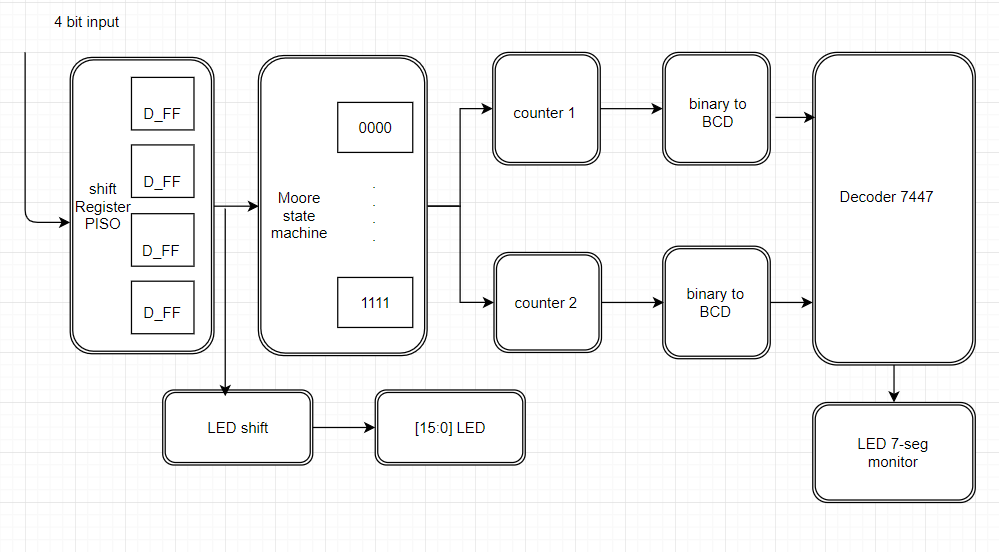
\includegraphics[width=15cm]{block_diagram.png}\\
Hình trên mô tả sơ đồ khối của mạch.
	\subsection{Shift register PISO}
	Khối này có chức năng là 1 thanh ghi dịch bao gồm 4 khối D Flip flop để 4 bit chứa dữ liệu nhập vào từ các switch 3 đến 0.\\ 
	
	Đồng thời khối này sẽ đẩy từng bit vào bộ xử lý chuỗi để phát hiện vị trí chuỗi mẫu.
	\subsection{Moore state machine}
	Kiểm tra dữ liệu chuyển từ thanh ghi dịch có phù hợp với chuỗi mẫu hay không.\\
	\subsection{counter1}
	Đếm vị trí của chuỗi con trong văn bản.
	\subsection{counter2}
	Đếm số chuỗi tìm được
	\subsection{binary to BCD}.
	Chuyển từ nhị phân sang BCD
	\subsection{Decode 7447}
	Giải mã để hiển thị ra màn hình Led 7 đoạn.
	\subsection{LEDshift}
	Hiển thị 18 ký tự mới nhất của đoạn văn bản trên 18 LED đỏ của board. 

%%%%%%%%%%%%%%%%%%%%%%%%%%%%%%%%%
\section{Hiện thực}
	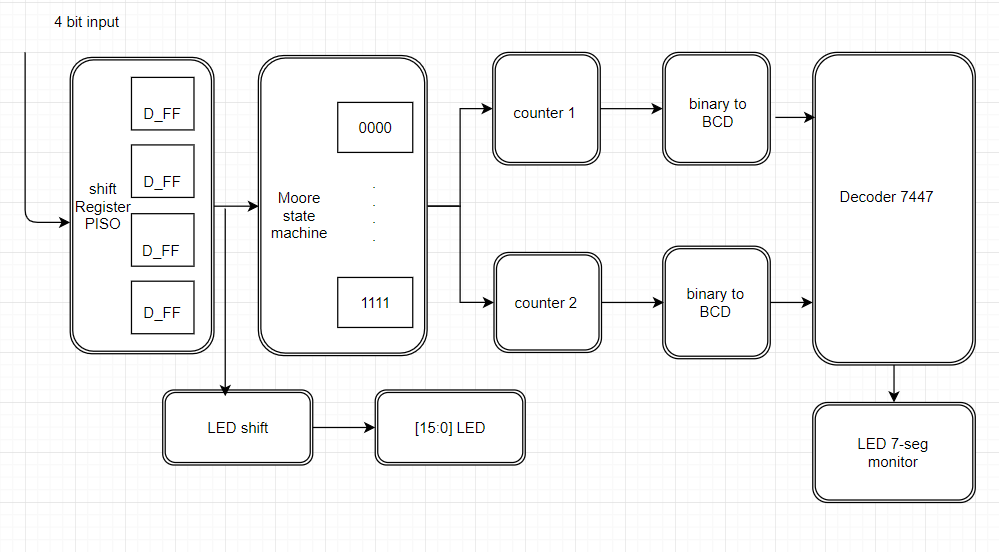
\includegraphics[width=15cm]{block_diagram.png}\\
	Hình trên mô tả sơ đồ khối của mạch.
	\subsection{Shift register PISO}
	
	Dưới đây là đoạn code Verilog mô tả thanh ghi dịch và cũng như các D Flip-Flop viết theo mô hình hành vi.\\
	
	Tín hiệu so là tín hiệu đầu ra chứa giá trị của các bit trong đoạn văn bản.
	
	B là đầu vào từ các SW[3:0]
	
	CLK là clock cho việc dịch/load thanh ghi.
	\begin{center}
	\begin{figure}[htp]
		\begin{center}
			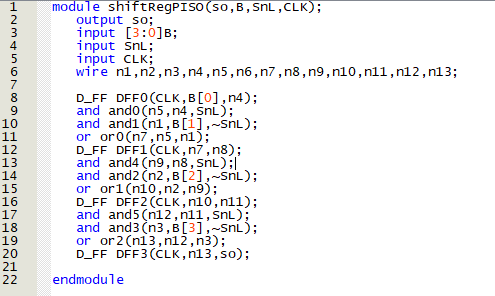
\includegraphics[scale=1]{shiftRegPISO.png}
		\end{center}
	\end{figure}
	\end{center}
	\begin{center}
	\begin{figure}[htp]
		\begin{center}
			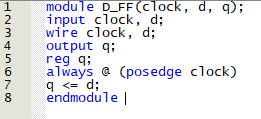
\includegraphics[scale=1.5]{Capture.png}
		\end{center}
	\end{figure}
	\end{center}
	
	\subsection{Moore state machine}
	Thiết kế bao gồm 16 máy trạng thái tương ứng với16 chuỗi 4 bit với cùng dữ kiệu vào và chọn 1 trong 16 dữ liệu ra.
	
	Dưới đây là đoạn code Verilog.\\
	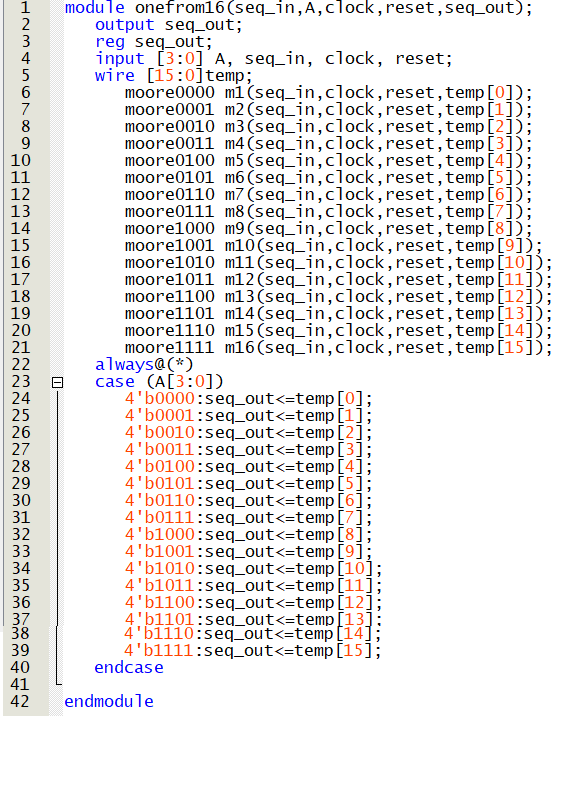
\includegraphics{onefrom16.png}
	
	Các module được thiết kế với sơ đồ trạng thái như sau:
	\newpage
%	
%	\begin{center}
%	\begin{figure}[htp]
%		\begin{center}
%			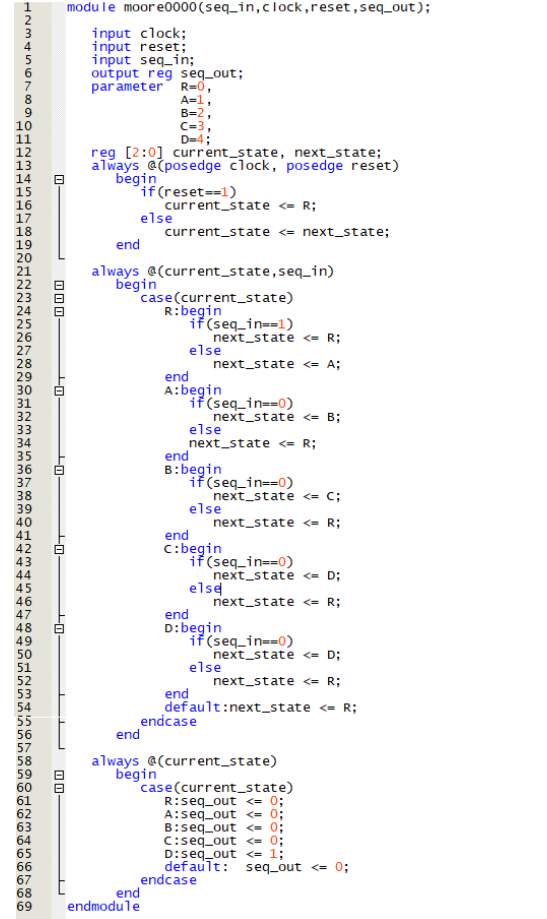
\includegraphics[scale=1]{02.png}
%		\end{center}
%	\end{figure}
%	\end{center}	
%	


	
	Sơ đồ trạng thái của chuỗi 0000
	\begin{center}
	\begin{figure}[h]
		\begin{center}
			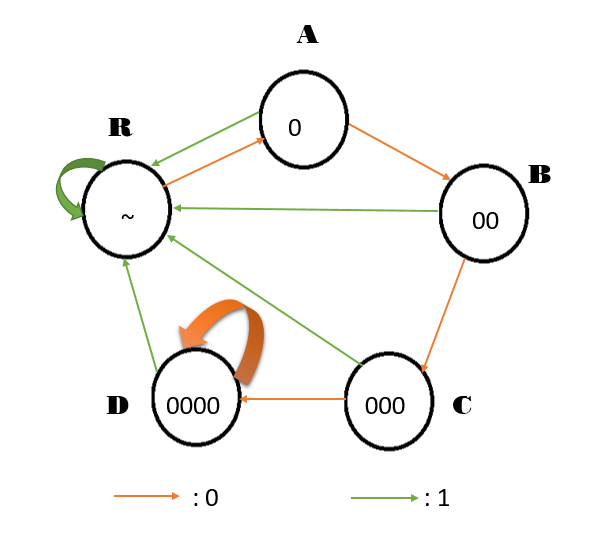
\includegraphics[scale=0.53]{0000.png}
		\end{center}
	\end{figure}
	\end{center}
	
	Sơ đồ trạng thái của chuỗi 0001
	\begin{center}
	\begin{figure}[h]
		\begin{center}
			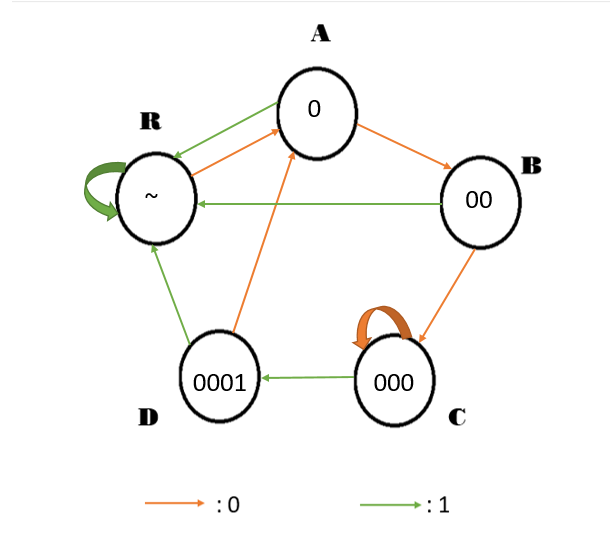
\includegraphics[scale=0.53]{0001.png}
		\end{center}
	\end{figure}
	\end{center}
	\newpage
	Sơ đồ trạng thái của chuỗi 0010
	\begin{center}
	\begin{figure}[h]
		\begin{center}
			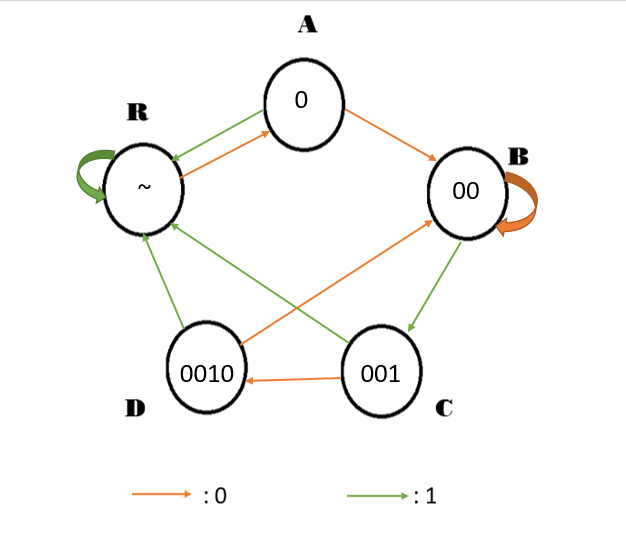
\includegraphics[scale=0.53]{0010.png}
		\end{center}
	\end{figure}
	\end{center}

		Sơ đồ trạng thái của chuỗi 0011
	\begin{center}
	\begin{figure}[h]
		\begin{center}
			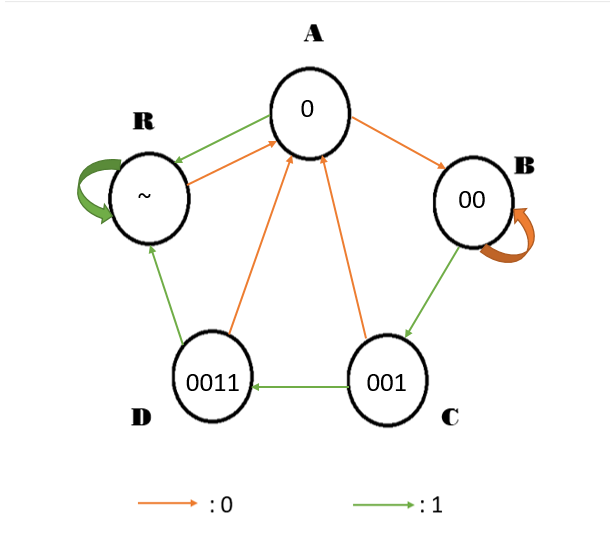
\includegraphics[scale=0.53]{0011.png}
		\end{center}
	\end{figure}
	\end{center}
	\newpage
	Sơ đồ trạng thái của chuỗi 0100
	\begin{center}
	\begin{figure}[h]
		\begin{center}
			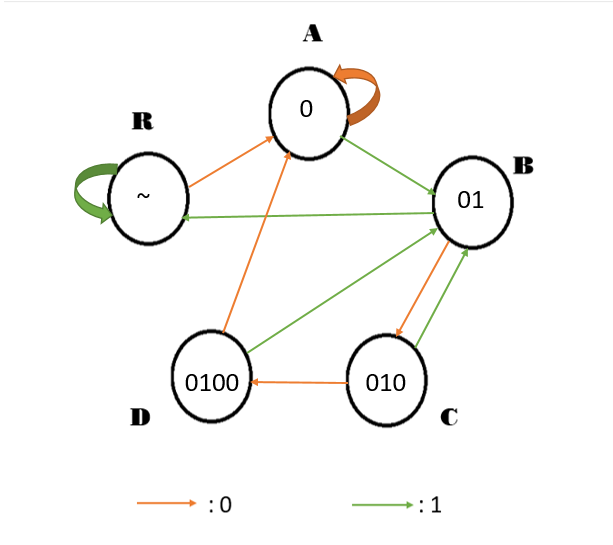
\includegraphics[scale=0.53]{0100.png}
		\end{center}
	\end{figure}
	\end{center}
	
		Sơ đồ trạng thái của chuỗi 0101
	\begin{center}
	\begin{figure}[h]
		\begin{center}
			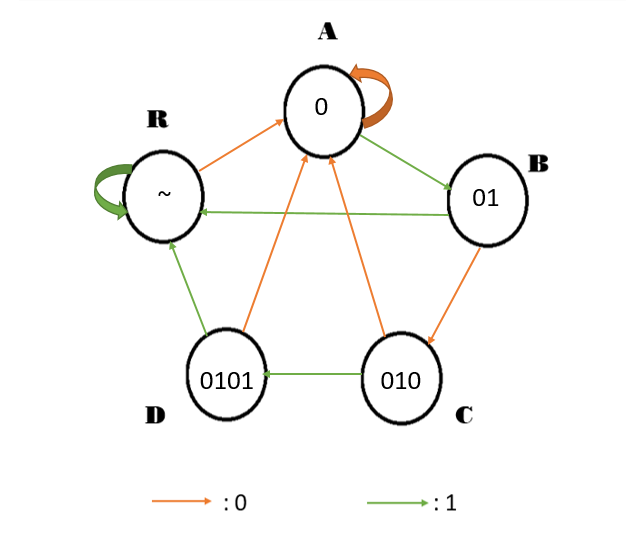
\includegraphics[scale=0.53]{0101.png}
		\end{center}
	\end{figure}
	\end{center}
	\newpage
	Sơ đồ trạng thái của chuỗi 0110
	\begin{center}
	\begin{figure}[h]
		\begin{center}
			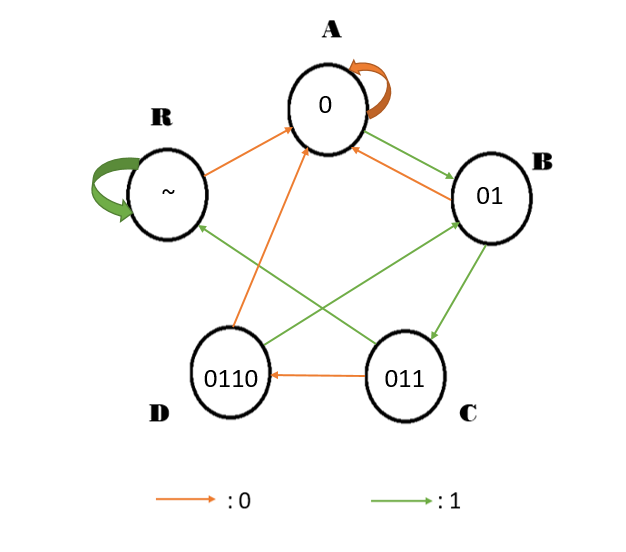
\includegraphics[scale=0.53]{0110.png}
		\end{center}
	\end{figure}
	\end{center}
	
		Sơ đồ trạng thái của chuỗi 0111
	\begin{center}
	\begin{figure}[h]
		\begin{center}
			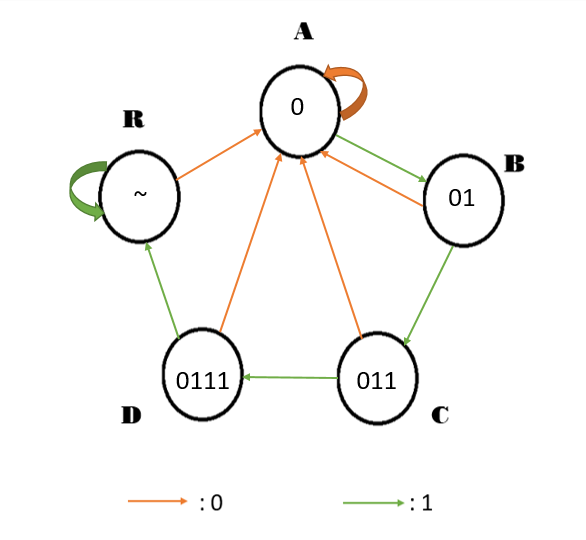
\includegraphics[scale=0.53]{0111.png}
		\end{center}
	\end{figure}
	\end{center}
	\newpage
	Sơ đồ trạng thái của chuỗi 1000
	\begin{center}
	\begin{figure}[h]
		\begin{center}
			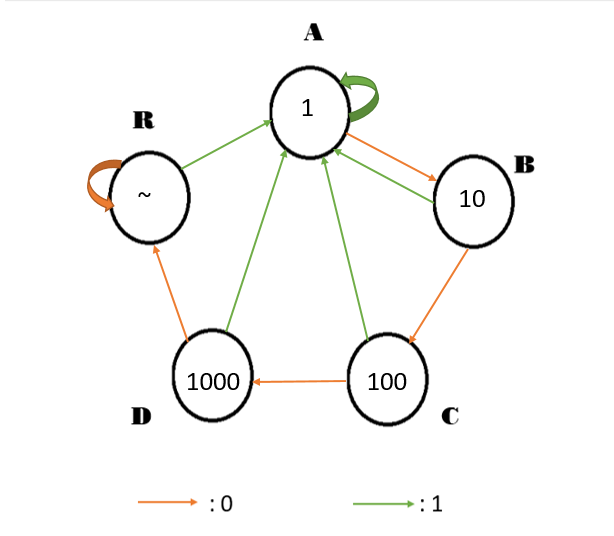
\includegraphics[scale=0.53]{1000.png}
		\end{center}
	\end{figure}
	\end{center}
	
		Sơ đồ trạng thái của chuỗi 1001
	\begin{center}
	\begin{figure}[h]
		\begin{center}
			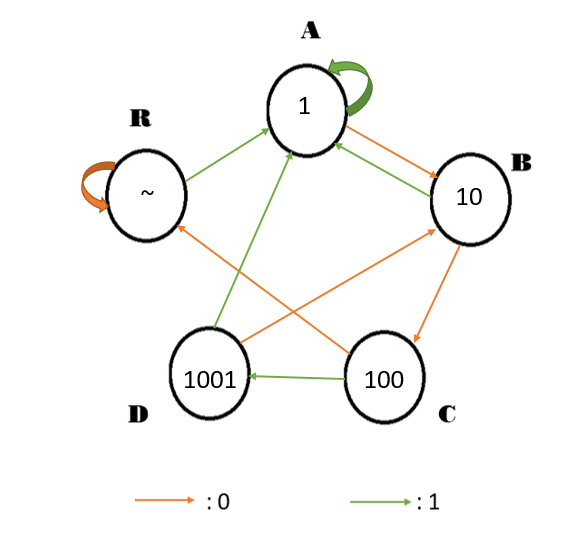
\includegraphics[scale=0.53]{1001.png}
		\end{center}
	\end{figure}
	\end{center}
	\newpage
	Sơ đồ trạng thái của chuỗi 1010
	\begin{center}
	\begin{figure}[h]
		\begin{center}
			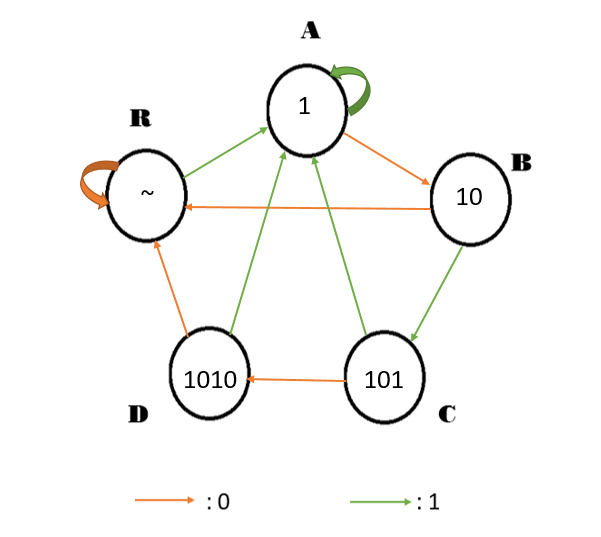
\includegraphics[scale=0.53]{1010.png}
		\end{center}
	\end{figure}
	\end{center}
	
		Sơ đồ trạng thái của chuỗi 1011
	\begin{center}
	\begin{figure}[h]
		\begin{center}
			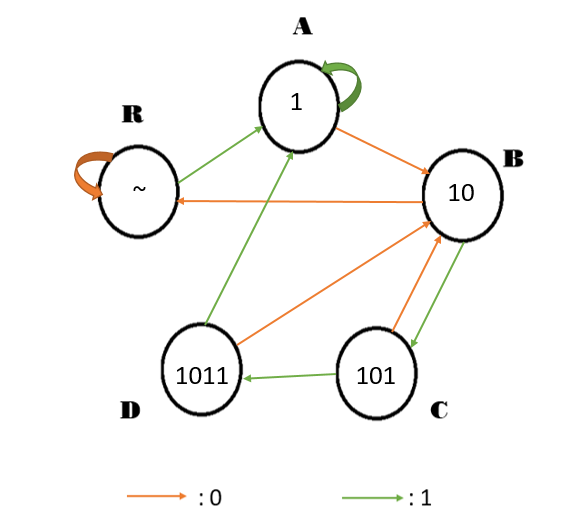
\includegraphics[scale=0.53]{1011.png}
		\end{center}
	\end{figure}
	\end{center}
	\newpage
	Sơ đồ trạng thái của chuỗi 1100
	\begin{center}
	\begin{figure}[h]
		\begin{center}
			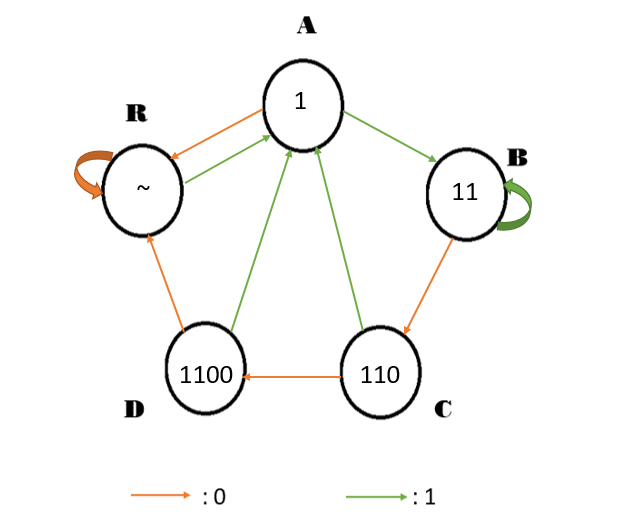
\includegraphics[scale=0.53]{1100.png}
		\end{center}
	\end{figure}
	\end{center}
	
		Sơ đồ trạng thái của chuỗi 1101
	\begin{center}
	\begin{figure}[h]
		\begin{center}
			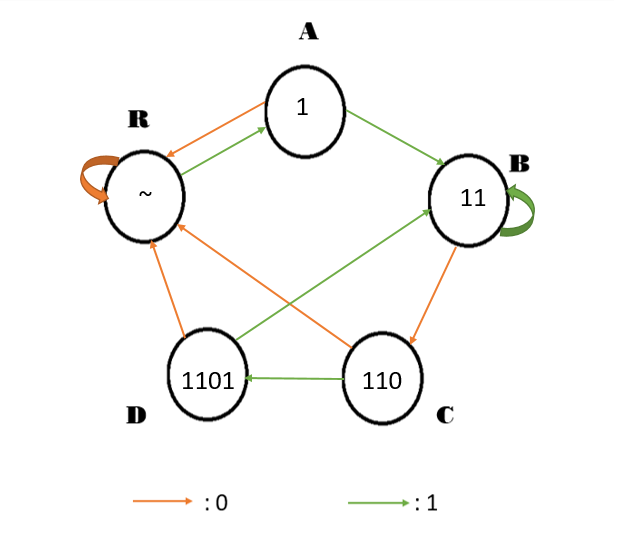
\includegraphics[scale=0.53]{1101.png}
		\end{center}
	\end{figure}
	\end{center}
	\newpage
	Sơ đồ trạng thái của chuỗi 1110
	\begin{center}
	\begin{figure}[h]
		\begin{center}
			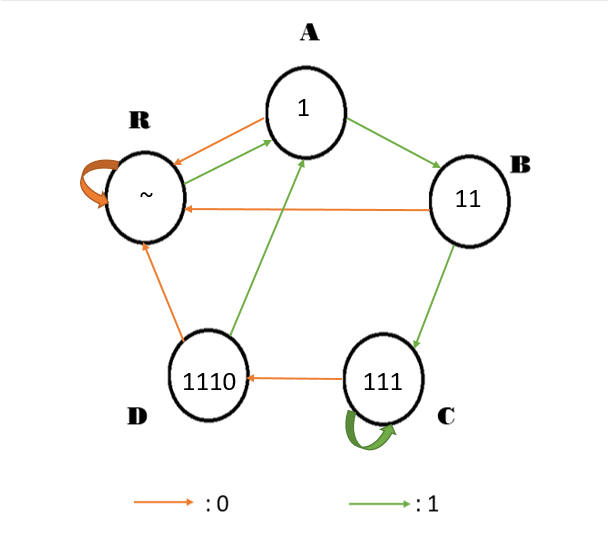
\includegraphics[scale=0.53]{1110.png}
		\end{center}
	\end{figure}
	\end{center}
	
	
	Sơ đồ trạng thái của chuỗi 1111
	\begin{center}
	\begin{figure}[h]
		\begin{center}
			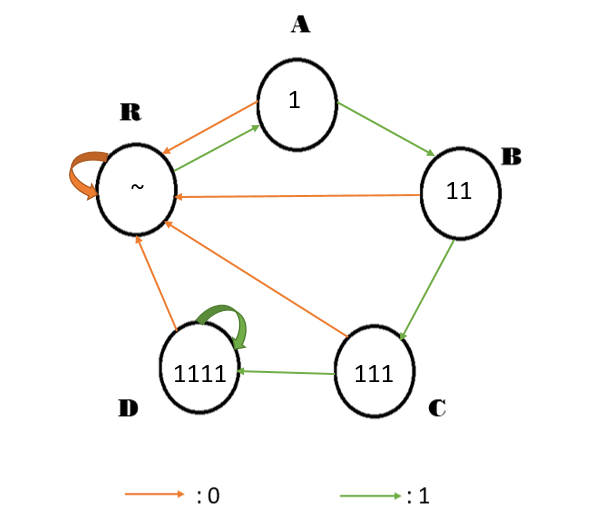
\includegraphics[scale=0.53]{1111.png}
		\end{center}
	\end{figure}
	\end{center}
		
	Dưới đây là ví dụ mẫu code Verilog bằng mô hình hành vi.\cite{bib2}
	
	\newpage
	\begin{center}
	\begin{figure}[H]
		\begin{center}
			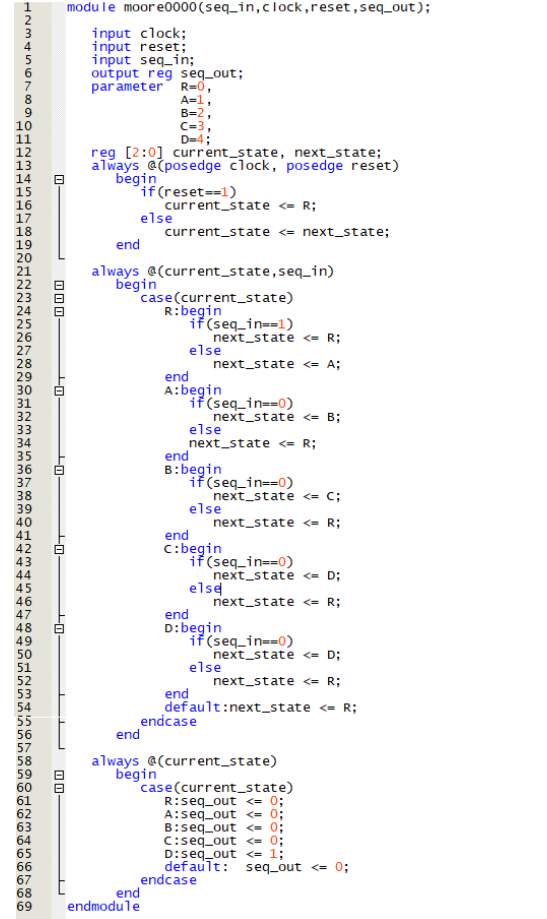
\includegraphics[scale=.8] {02.png}
		\end{center}
	\end{figure}
	\end{center}	
	\newpage
	
	\subsection{counter 1}
	
	Dưới đây là đoạn code verilog, được viết theo mô hình hành vi
	
	\begin{center}
	\begin{figure}[H]
		\begin{center}
			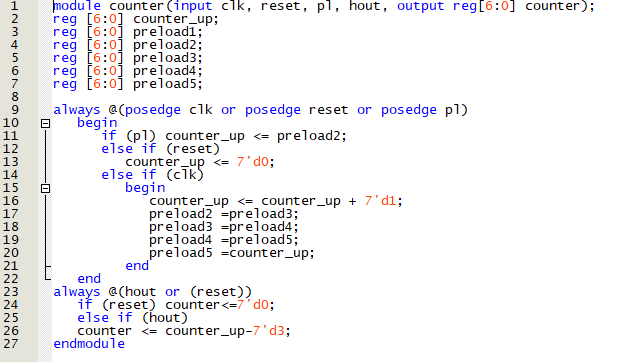
\includegraphics[scale=.8] {c.png}
		\end{center}
	\end{figure}
	\end{center}	
	
	\subsection{counter 2}
	
	Dưới đây là đoạn code verilog, được viết theo mô hình hành vi
	
	\begin{center}
	\begin{figure}[H]
		\begin{center}
			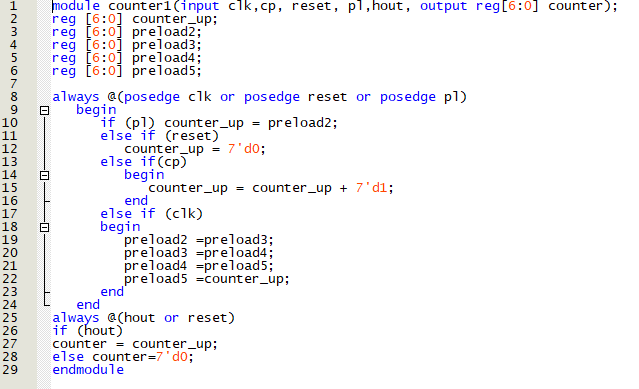
\includegraphics[scale=.83] {c1.png}
		\end{center}
	\end{figure}
	\end{center}	
	
	\subsection{bin to BCD}
	Chuyển dữ liệu đầu vào là số nhị phân 7 bit sang mã BCD bằng giải thuật DOuble Dabble, tức là dịch dần 7 bit sang trái và so sánh các cột 4 bit với 5. Nếu lớn hơn 5 thì cộng thêm ba vào cho đến khi dịch hết 7 bit.  
	
	Đoạn code sau được viết theo mô hình hành vi mô phỏng giải thuật trên.\cite{bib3}
	
	\begin{center}
	\begin{figure}[H]
		\begin{center}
			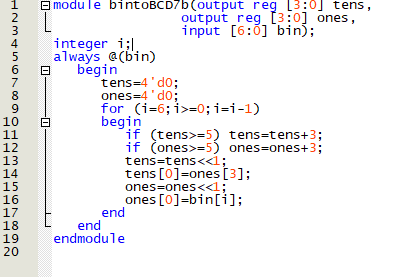
\includegraphics[scale=.83] {b.png}
		\end{center}
	\end{figure}
	\end{center}
	
	\subsection{Decode 7447}
	Mô phỏng lại hoạt động của ic 7447, tức là giải mã soos4 bit để đưa vào LED 7 đoạn
	
	Đoạn code sau được viết theo mô hình RTL
	
	\begin{center}
	\begin{figure}[H]
		\begin{center}
			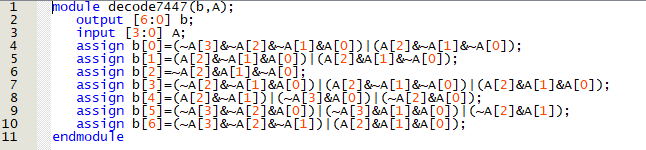
\includegraphics[scale=.83] {de.png}
		\end{center}
	\end{figure}
	\end{center}  
	\subsection{LEDshift}
	Điều khiển hiển thị cac LED đỏ biểu diễn 18 ký tự gần nhất của văn bản
	
	\begin{center}
	\begin{figure}[H]
		\begin{center}
			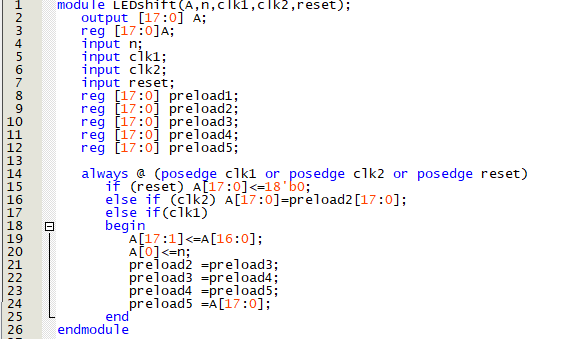
\includegraphics[scale=.83] {l.png}
		\end{center}
	\end{figure}
	\end{center}  
	
%%%%%%%%%%%%%%%%%%%%%%%%%%%%%%%%%
\section{Kiểm thử}
Kiểm thử hệ thống trên board De2i-150:
	\begin{center}
	\begin{figure}[H]
		\begin{center}
			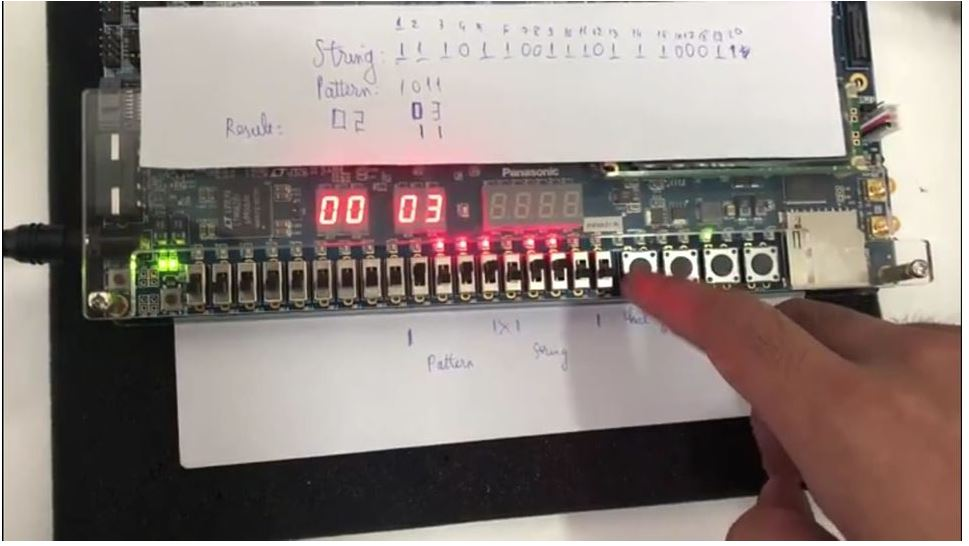
\includegraphics[scale=.5] {k2.jpg}
		\end{center}
	\end{figure}
	\end{center}  
	
	\begin{center}
	\begin{figure}[H]
		\begin{center}
			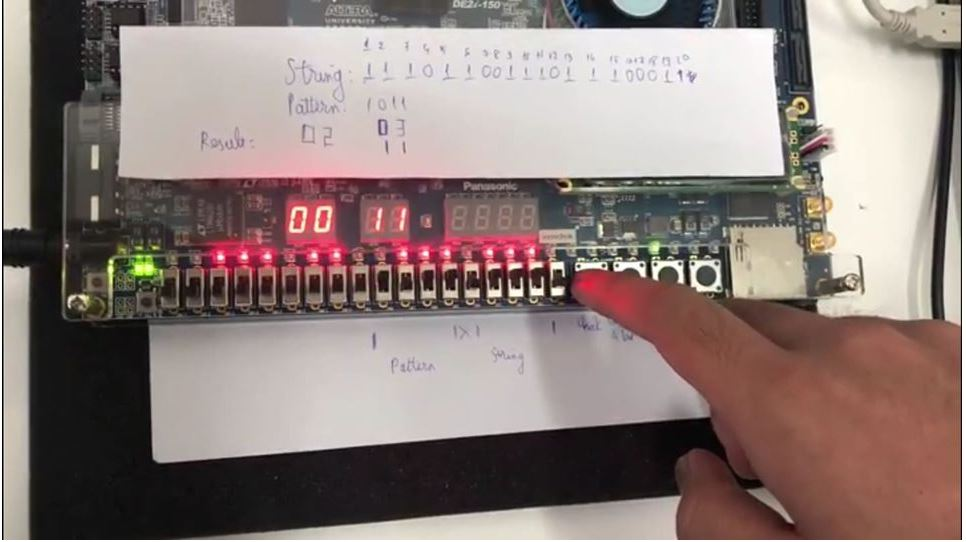
\includegraphics[scale=.5] {k1.jpg}
		\end{center}
	\end{figure}
	\end{center}  
	
	\begin{center}
	\begin{figure}[H]
		\begin{center}
			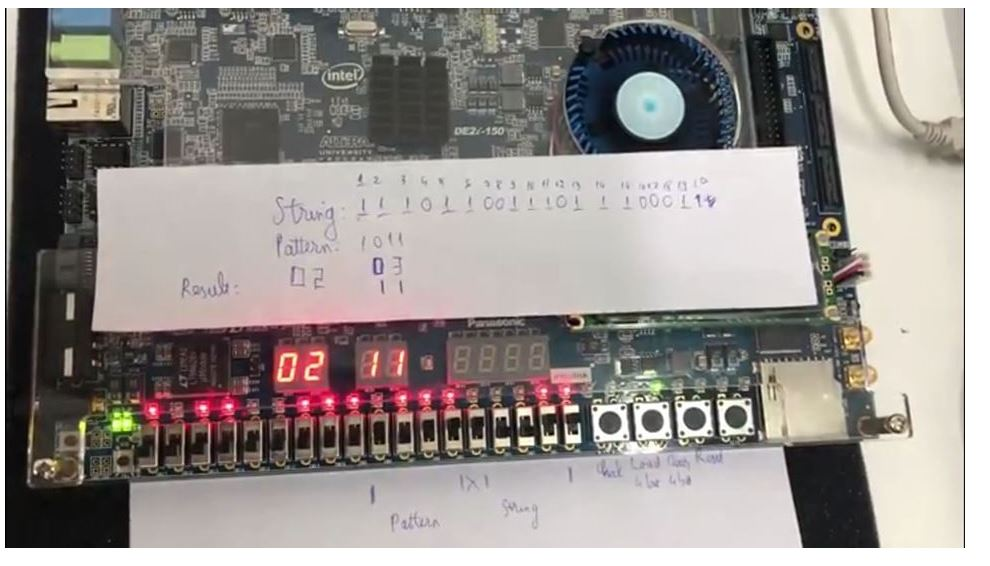
\includegraphics[scale=.5] {k3.jpg}
		\end{center}
	\end{figure}
	\end{center}  
\begin{center}
	\begin{figure}[H]
		\begin{center}
			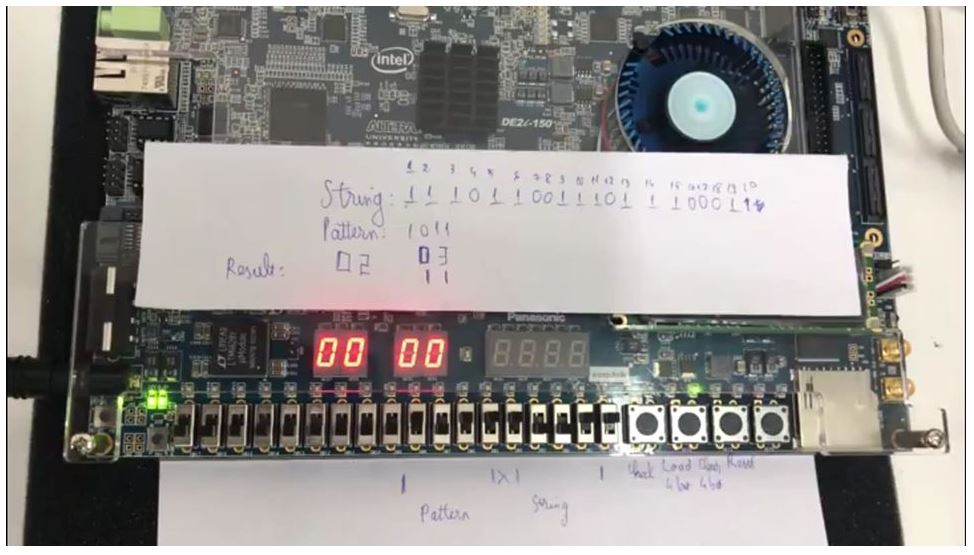
\includegraphics[scale=.5] {k9.jpg}
		\end{center}
	\end{figure}
	\end{center}  	
	
	\begin{center}
	\begin{figure}[H]
		\begin{center}
			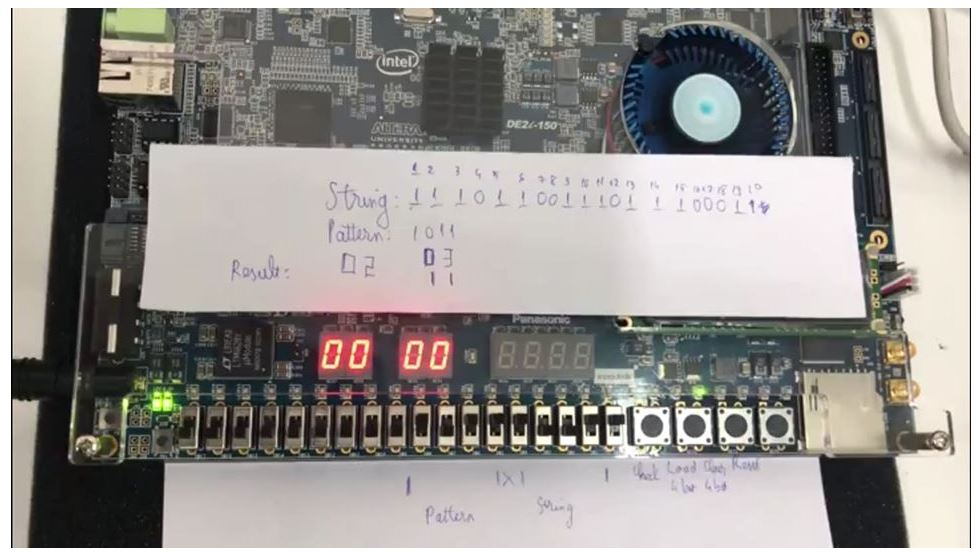
\includegraphics[scale=.5] {k8.jpg}
		\end{center}
	\end{figure}
	\end{center}  
	
	\begin{center}
	\begin{figure}[H]
		\begin{center}
			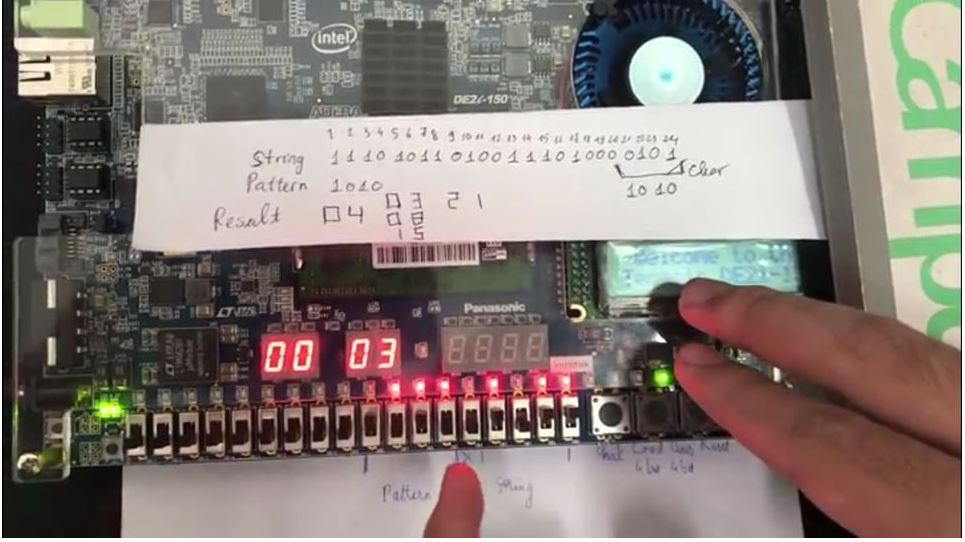
\includegraphics[scale=.5] {k4.jpg}
		\end{center}
	\end{figure}
	\end{center}  
	
	\begin{center}
	\begin{figure}[H]
		\begin{center}
			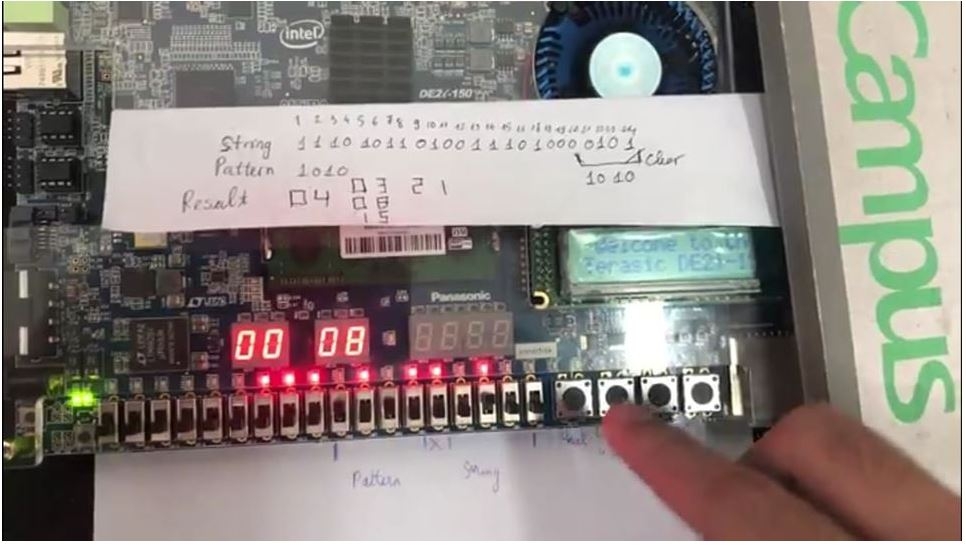
\includegraphics[scale=.5] {k5.jpg}
		\end{center}
	\end{figure}
	\end{center}  
	
	\begin{center}
	\begin{figure}[H]
		\begin{center}
			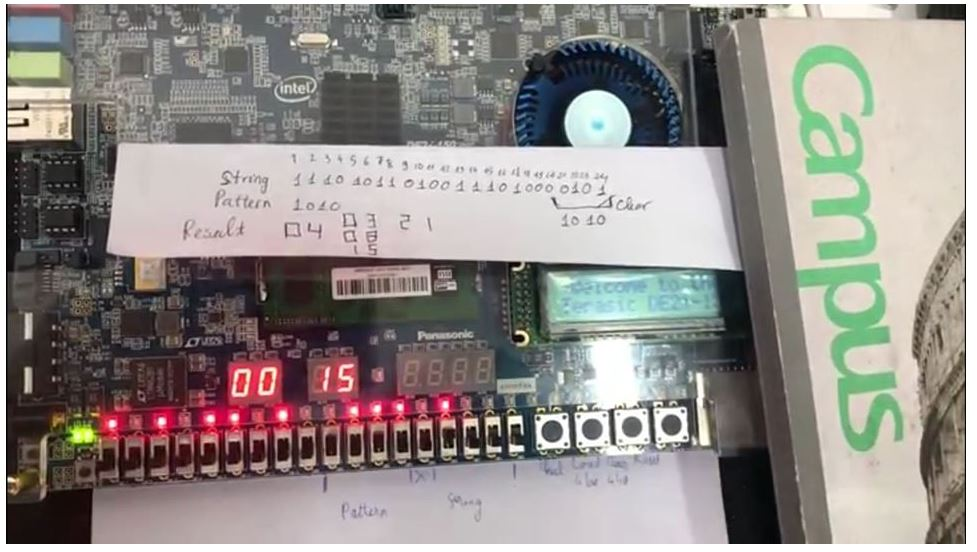
\includegraphics[scale=.5] {k6.jpg}
		\end{center}
	\end{figure}
	\end{center}  
	
	\begin{center}
	\begin{figure}[H]
		\begin{center}
			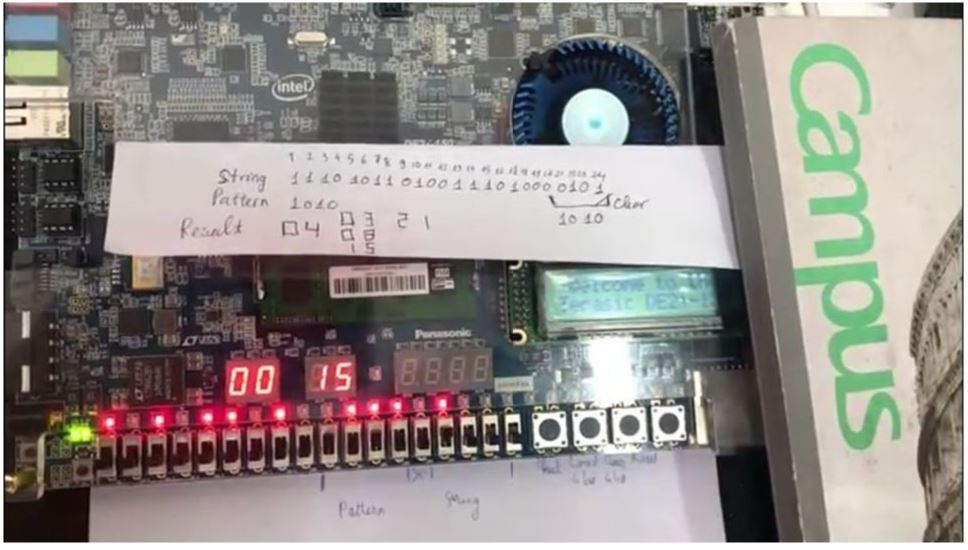
\includegraphics[scale=.5] {k7.jpg}
		\end{center}
	\end{figure}
	\end{center}  
%%%%%%%%%%%%%%%%%%%%%%%%%%%%%%%%%
\section{Kết luận}
	
Hệ thống phát hiện chuỗi có rất nhiều ứng dụng trong kỹ thuật xử lý tín hiệu. Trên đây nhóm 5 đã trình bày Các bước xây dựng một hệ thông phát hiện chuỗi đơn giản mà nhóm đã tìm hiểu được, đồng thời mô phognr nó trên Board Altera De2i-150.

Qua đó, nhóm đã gặp phải một số khó khăn, chủ yếu ở việc lưu các trạng thái qua mỗi clock để có thể quay lại khi chuỗi bị xoá. Về vấn đề này, nhóm vẫn chưa thể hiện thực hoàn hảo được.

Trong tương lai, nếu có cơ hội, nhóm 5 sẽ cùng nhau thảo luận và đưa ra các giải pháp cải tiến hệ thống, về giao diện với người dùng cũng như các tính năng như xoá các chuỗi con ra khỏi đoạn văn bản hoặc thay đổi cỡ chuỗi mẫu (pattern). Trên hết cả, nhóm sẽ cố gắng hiện thực hoá hệ thống này, không phải trên Board Altera De2i-150 mà là một hệ thống thực sự với đầy đủ phần cứng 

%%%%%%%%%%%%%%%%%%%%%%%%%%%%%%%%%

\section{Bảng phân công công việc}
\begin{tabular}{ |l|l|}
\hline
  Nguyễn Trần Quang Minh & Thiêt kế các module Moore state machine và LEDshift \\
  \hline
  Nguyễn Duy Sơn & Thiết kế các module counter1, counter2, bin to BCD, Decode 7447\\
\hline  
  Võ Ngọc Quý &  Thiết kế Shift register PISO và viết báo cáo\\
\hline  
  Mai Đình Phúc &  Hỗ trợ viết báo cáo (Hình ảnh minh hoạ)\\
\hline  
  Nguyễn Đức Lộc & Slide thuyết trình \\
\hline  
  Nguyễn Ngọc Lan Anh & Slide thuyết trình \\
  \hline
\end{tabular}

\begin{thebibliography}{80}


\bibitem{bib1} Tocci, R.J. (2007).\textit{Digital systems: principles and applications}.	Prentice Hall PTR, 1988.
\bibitem{bib2} \href{https://www.fpga4student.com/2017/09/verilog-code-for-moore-fsm-sequence-detector.html}{FPGA for Students}
\bibitem{bib3} \href{https://en.wikipedia.org/wiki/Double_dabble}{Wikipedia contributors. (2019, May 12). Double dabble. In Wikipedia, The Free Encyclopedia}
\end{thebibliography}
\end{document}

